\documentclass[11pt,openright,a4paper]{article}
\usepackage{fancyhdr}
\usepackage{datetime}
\usepackage[left=25mm,right=25mm,top=35mm,bottom=35mm,footskip=0.5in]{geometry}
% %%
%% Package includes to provide the basic style
%%
\usepackage{harvard}    % Uses harvard style referencing
\usepackage{graphicx}   % Permits import of various graphics formats
\usepackage{hyperref}   % Provides hyperlinks to sections automatically
\usepackage{pdflscape}  % Provides landscape mode for end code listings
\usepackage{multicol}   % Provides ability to split output into columns
\usepackage{listings}   % Provides styled code listings
\usepackage{titlesec}
\usepackage[margin=35mm,footskip=0.5in]{geometry}
\usepackage{tabularx}
\usepackage{tabulary}
\usepackage{multirow}
\usepackage{color}
\usepackage[table]{xcolor}
\usepackage{caption, subcaption}
\usepackage{amssymb, amsmath, empheq}
\lstset{language=Python}
\usepackage{array}
\usepackage{longtable}
\usepackage{subfiles}
\usepackage{float}
\usepackage{longtable}

\graphicspath{ {images/} {lit_review/images/} {images/tech/} {images/methodology/} {images/results/} }
% \numberwithin{equation}{chapter}

\let\subsectionautorefname\sectionautorefname
\let\subsubsectionautorefname\sectionautorefname

% % set margin
% \geometry{
%   a4paper,
%   top=25mm,
%   bottom=35mm
% }

%%
%% Set some page size changes from the standard article class
%%
\usepackage{calc}
\setlength{\parskip}{6pt}
\setlength{\parindent}{0pt}
\addtolength{\hoffset}{0.5cm}
\addtolength{\textwidth}{0.5cm}

% set section depth
\setcounter{tocdepth}{4}
\setcounter{secnumdepth}{5}

% set chapter format
%\titleformat{\chapter}[hang]{\LARGE\bfseries}{\thechapter\hspace{20pt}}{0pt}{\LARGE\bfseries}
%\titlespacing{\chapter}{0pt}{0pt}{5pt}

%%
%% Format definitions for the style
%%
\bibliographystyle{agsm}  %{alpha}
\citationstyle{dcu}
\pagestyle{headings}
\fussy


%%
%% Definitions to provide layout in the dissertation title pages
%%
\newenvironment{spaced}[1]
  {\begin{minipage}[c]{\textwidth}\vspace{#1}}
  {\end{minipage}}


\newenvironment{centrespaced}[2]
  {\begin{center}\begin{minipage}[c]{#1}\vspace{#2}}
  {\end{minipage}\end{center}}


%%
%% New column header command
%% 
\newcolumntype{Z}{ >{\centering\arraybackslash}X }
\newcolumntype{M}[1]{ >{\centering\arraybackslash}m{#1}}


% declaration
\newcommand{\declaration}[2]{
  \thispagestyle{empty}
  \begin{spaced}{4em}
    \begin{center}
      \LARGE\textbf{#1}
    \end{center}
  \end{spaced}
  \begin{spaced}{3em}
    \begin{center}
      Submitted by: #2
    \end{center}
  \end{spaced}
  \begin{spaced}{5em}
    \section*{COPYRIGHT}

    Attention is drawn to the fact that copyright of this dissertation rests
    with its author. The Intellectual Property Rights of the products
    produced as part of the project belong to the author unless otherwise specified
    below, in accordance with the University of Bath's policy on intellectual property 
   (see http://www.bath.ac.uk/ordinances/22.pdf).

    This copy of the dissertation has been supplied on condition that anyone
    who consults it is understood to recognise that its copyright rests with its
    author and that no quotation from the dissertation and no information
    derived from it may be published without the prior written consent of
    the author. \\ \\

    \section*{DECLARATION}
    This dissertation is submitted to the University of Bath in accordance
    with the requirements of the degree of Bachelor of Science in the
    Department of Computer Science. No portion of the work in this dissertation
    has been submitted in support of an application for any other degree
    or qualification of this or any other university or institution of learning.
    Except where specifically acknowledged, it is the work of the author.
  \end{spaced}

  \begin{spaced}{5em}
    Signed:
  \end{spaced}
  }


% consultation
\newcommand{\consultation}[1]{%
\thispagestyle{empty}
\begin{centrespaced}{0.8\textwidth}{0.4\textheight}
\ifnum #1 = 0
This dissertation may be made available for consultation within the
University Library and may be photocopied or lent to other libraries
for the purposes of consultation.
\else
This dissertation may not be consulted, photocopied or lent to other
libraries without the permission of the author for #1 
\ifnum #1 = 1
year
\else
years
\fi
from the date of submission of the dissertation.
\fi
\vspace{4em}

Signed:
\end{centrespaced}
}

%%
%% END OF DEFINITIONS
%%


\usepackage{amsmath}
\usepackage{hyperref}
\usepackage{amsbsy}
\usepackage{graphicx}
\usepackage{float}

\usepackage[english]{babel}
\usepackage[backend=bibtex,sorting=none,style=ieee]{biblatex}
\bibliography{task3bib}

\graphicspath{ {images/} }
\usepackage{graphicx}

% header
\pagestyle{fancy}
\fancyhf{}
\lhead{CM50426 Machine Learning \& AI \\ Alan Lau}
\rhead{Task 3 \\ Semester 1, 2016-17}
\cfoot{\thepage}

\setlength{\parindent}{0em}
\setlength{\parskip}{1em}
\numberwithin{equation}{section}

\abovedisplayskip=12pt plus 3pt minus 9pt
\abovedisplayshortskip=0pt plus 3pt
\belowdisplayskip=12pt plus 3pt minus 9pt
\belowdisplayshortskip=7pt plus 3pt minus 4pt

\usepackage[font=small,labelfont=bf]{caption}


% define a macro \Autoref to allow multiple references to be passed to \autoref
\newcommand\Autoref[1]{\@first@ref#1,@}
\def\@throw@dot#1.#2@{#1}% discard everything after the dot
\def\@set@refname#1{%    % set \@refname to autoefname+s using \getrefbykeydefault
    \edef\@tmp{\getrefbykeydefault{#1}{anchor}{}}%
    \def\@refname{\@nameuse{\expandafter\@throw@dot\@tmp.@autorefname}s}%
}
\def\@first@ref#1,#2{%
  \ifx#2@\autoref{#1}\let\@nextref\@gobble% only one ref, revert to normal \autoref
  \else%
    \@set@refname{#1}%  set \@refname to autoref name
    \@refname~\ref{#1}% add autoefname and first reference
    \let\@nextref\@next@ref% push processing to \@next@ref
  \fi%
  \@nextref#2%
}
\def\@next@ref#1,#2{%
   \ifx#2@ and~\ref{#1}\let\@nextref\@gobble% at end: print and+\ref and stop
   \else, \ref{#1}% print  ,+\ref and continue
   \fi%
   \@nextref#2%
}


\begin{document}

% - Differences between ML, MAP and Bayesian
    % - suitability, pros and cons
    % - how to pick a model to use based on the data
% - What is meant by overfitting in non-linear
% - How to initialise the models

% - Why does the method work, and when
% - How efficient is the method (accuracy VS computational expensiveness)
% - Compare with other methods
% - How could I improve it

%%%%%%%%%%%%%
\section{Introduction} \label{sec:intro}
%%%%%%%%%%%%%
Supervised learning uses datapoints with correpsonding target vectors to train a model. In general, we aim to create a model such that datapoints are assigned to a finite number of categories, which is bounding by the set of unique target vectors. The simplest case would be a binary classifier where we learn from a dataset of feature-target pairs in order to decide whether a datapoint belongs to a particular class.

%%%%%%%%%%%%
\section{Discriminative \textit{vs} Generative Model} \label{sec:types}
%%%%%%%%%%%%
There are two types of supervised classifier models, namely discriminative and generative.

For a discriminative model, we aim to model the contingency of the world state on the data, i.e. $Pr\left(\mathbf{w} | \mathbf{x}\right)$. It aims to learn the the boundaries that split between classes, so that one may distinguish datapoints of one class from another.

For a generative model, we aim to model the contingency of the data on the world state, i.e. $Pr \left(\mathbf{x} | \mathbf{w} \right)$. By learning the distribution of each class, new datapoints can be generated by referring to the distribution.

The learning process of the two types of models is similar:
\begin{enumerate}
    \item We first choose an appropriate form for $Pr(\mathbf{w})$ (discriminative) or $Pr(\mathbf{x})$) (generative). 
    \item Then, parameters are made a function of $\mathbf{x}$ (discriminative) or $\mathbf{w}$ (generative). 
    \item These functions take appropriate parameters $\boldsymbol{\theta}$, which are learnt using standard methods such as maximum likelihood and MAP. 
\end{enumerate}

The differences between the two methods start with inferencing. Inference is performed simply through evaluating $Pr(\mathbf{w}|\mathbf{x})$ for a discriminative model. For a generative model, we first have to define a prior $Pr(\mathbf{w})$ before computing the posterior $Pr(\mathbf{w}|\mathbf{x})$ with Bayes rule, which makes it more difficult than that of a discriminative model.

A generative model more closely models the real world. It enables prior knowledge to be taken into account, so that some known facts do not have to be relearnt. This is much more difficult in a discriminative model. Also, we do not usually have perfect data. Since it learns the joint distribution over all dimensions, it can interpolate and fill in the missing data.

However, by learning across all dimensions, a generative model is costly to train especially on a dataset of high dimensionality, where most of these dimensions may not even influence the state after all. 


%%%%%%%%%%%%
\section{Naive Bayes Classifier (Generative)} \label{sec:gen}
%%%%%%%%%%%%

%TODO: include image of the distribution shapes


\begin{equation} \label{eq:gen-likelihood}
    Pr \left ( x | w \right ) = \text{Norm}_x \left [ \mu_w, \sigma_{w}^{2}  \right ]
\end{equation}

Consider a classifer that uses 1 to represent present and 0 otherwise, i.e. the label $w \in \{0,1\}$ to represent this. Following the steps in \autoref{sec:types}, we choose the Guassian distribution for $Pr(\mathbf{x})$. Hence, we have the likelihood as \autoref{eq:gen-likelihood}, taking parameters $\mu_0$, $\mu_1$, $\sigma_{0}^{2}$, $\sigma_{1}^{2}$, which defines its shape.

\begin{equation} \label{eq:gen-params}
    \begin{aligned}
        \hat{\mu_{w}} &= \frac{1}{N_{w}} \sum_{n=1}^{N_w} x_n
        \\
        \hat{\Sigma_w} &= \frac{1}{N_w} \sum_{n=1}^{N_w} \left ( x_n - \hat{\mu}  \right ) \left ( x_n - \hat{\mu} \right )^{T}
    \end{aligned}
\end{equation}

The parameters can be learnt through maximum likelihood as shown in \autoref{eq:gen-params}. The mean input for each label is simply the mean of its feature vectors, and similarly the covariance. This can be observed simply by taking the derivative of the log-likelihood function and equating it to zero.

% TODO: point out how this makes it generative


%TODO edit this given experiment (give code block positions)
Using the given \textit{test case 0} with default parameters, we can see that it achieved a perfect accuracy. The reason is that there is no overlap between the two classes, which makes it possible to predict with very high convidence the class of a datapoint. By increasing noise level and introducing overlapping datapoints, we can see that the accuracy starts to decrease. 

The code block, `Naive Bayes' in \textit{test.py} demonstrates this. Using 250 datapoints for each of the training and testing steps, we achieved a 100\% accuracy rate.


%%%%%%%%%%%%
\section{Linear Logistic Regression Classifier} \label{sec:lr}
%%%%%%%%%%%%
A logistic regression classifier is a discriminative method that selects a probability distribution over the world state $w \in \{0,1\}$ with its parameters a function of the training features $\mathbf{x}$. Since the world state is binary, we choose the Bernoulli distribution - $Pr(w | \boldsymbol{\phi}, \mathbf{x}) = \text{Bern}_w [\text{sig}[a]]$. Note that $\phi_0$ is prepended to $\boldsymbol{\phi}$ and similarly, 1 to the $\mathbf{x}$.

$a = \phi^T\mathbf{x}$ is the activation function. However, we could not simply use this as the parameter $\lambda$ for the classifier, as it would allow any value to be returned, but we require it to be between 0 and 1. Hence, we apply a the logistic sigmoid function that maps $[-\infty, \infty]$ to $[0, 1]$. The sigmoid function is given by 

\begin{equation} \label{eq:lr-sig}
    \text{sig} \left [ a \right ] = \frac{1}{1 + \text{exp} \left [ -a \right ] }
\end{equation}

\begin{equation} \label{eq:lr-prob}
    \begin{aligned}
        Pr \left ( \mathbf{w} | \mathbf{X}, \phi \right ) &= 
            \prod_{i=1}^{I} \lambda^{w_i} \left (1-\lambda \right )^{1-w_i}
        \\
        &= \prod_{i=1}^{I} 
            \left ( 
                \frac{1}
                     {1 + \text{exp} \left [ -\phi^{T} \mathbf{x}_i \right ]}  
            \right )^{w_i}
            \left ( \frac{\text{exp} \left [ -\phi^{T} \mathbf{x}_i \right ]}
                         {1 + \text{exp} \left [ -\phi^{T} \mathbf{x}_i \right ]} 
            \right )^{1-w_i}
    \end{aligned}
\end{equation}

Given training data $\mathbf{X} = [x_1, ..., x_I]$, targets $\mathbf{w} = [w_1, ..., w_I]^T$ and the aforementioned parameters, we can compute the probability with \autoref{eq:lr-prob}. Now, we have to find the parameters $\phi$ using either ML or MAP.

\textit{Note: the ML and MAP equations are expressed in a way to be used by a \textbf{minimisation} algorithm, as opposed to maximisation.}

\subsection{Optimisation} \label{ssec:lr-op}
We need to use an iterative non-linear optimisation method to estimate the parameters for logistic regression classifiers, as we later see that it is not possible to evalute the derivatives in closed forms. We can iteratively find the mimum by using \textit{scipy}'s \textit{minimize} function.

Our goal is to find the parameters that minimise the objective function, i.e. $\hat{\boldsymbol\theta} = \text{argmin}_{\boldsymbol{\theta}} f[\boldsymbol\theta]$. 

\begin{equation} \label{eq:lr-op-newton}
    \boldsymbol\phi^{[t]} = \boldsymbol\phi^{[t+1]} + 
    \alpha \left ( \frac{\partial^2 L}{\partial \boldsymbol{\phi}^2} \right )^{-1}
    \frac{\partial L}{\partial \boldsymbol\phi}
\end{equation}

The basic idea is to start with an initial guess $\boldsymbol\phi^{[0]}$, then take small steps with subsequent guesses that decreases the cost/ objective function. We reach a minimum when no improvement can be made further. \autoref{eq:lr-op-newton} shows the Newton's Method, where both the first and second derivatives of L with respect to $\boldsymbol\phi$. 

The second derivative, known as the Hessian matrix, is used to check if the function is convex. A convex function has one minimum, otherwise we might obtain a local minimum instead. Other methods such as BFGS do not take it into account.


\subsection{Finding Parameters using Maximum Likelihood (ML)} \label{ssec:lr-ml}

\begin{equation} \label{eq:lr-ml-L}
    L = -\sum_{i=1}^{I} w_i \text{log} 
            \left [ \frac{1}
                         {1 + \text{exp} \left [ -\phi^{T} \mathbf{x}_i \right ]} \right ]
        -
        \sum_{i=1}^{I} \left (1-w_i \right ) \text{log} 
            \left [ \frac{\text{exp} \left [ -\phi^{T} \mathbf{x}_i \right ]}
                         {1 + \text{exp} \left [ -\phi^{T} \mathbf{x}_i \right ]} 
            \right ]
\end{equation}

To make computation easier and to allow a quicker convergence, we take logorithm on \autoref{eq:lr-prob} to obtain \autoref{eq:lr-ml-L}. We then take the first derivative of L with respect to the parameters $\phi$ to obatin the gradient. The second derivative gives the Hessian matrix, which provides curvature information for more accurate optimisation using methods such as Newton's Method. They are shown below in \autoref{eq:lr-ml-derv}.

\begin{equation} \label{eq:lr-ml-derv}
    \begin{aligned}
        \frac{\partial L}{\partial \phi} &= 
            \sum_{i=1}^{I} \left ( \text{sig} \left [ a_i  \right ] - w_i \right ) \mathbf{x}_i
        \\
        \frac{\partial^2 L}{\partial \phi^2} &=
            \sum_{i=1}^{I} \text{sig} \left [ a_i  \right ] 
                \left ( 1 - \text{sig} \left [ a_i  \right ] \right ) 
                \mathbf{x}_i \mathbf{x}_i^{T}
    \end{aligned}
\end{equation}

%TODO:Linear ML optimisation plots over all 3 sets

The limitation of using Maximum Likelihood for estimating the parameters is that the model becomes overconfident, as we do not consider a prior nor uncertainty. Also, the model could only describe the split between classes linearly, as seen in PICTURE that \textit{test case 1} and \textit{test case 2} do not work well under this model.

With linearly seperable datasets and at high dimensionality, this model can be easily overfitted. When $a = 0$, $\text{sig} [a]$ becomes infinitely steep, resulting in all training features will give a posterior probability of 1. This problem continues, as that there is no way for ML to choose a solution against another.

% TODO: different initialisation graphs

The solutions found by ML are also very dependent on parameter initialisation and the optimisation algorithm chosen given linearly seperable datasets. This will still occur no matter the ratio between the size of the dataset and the number of parameters.


%%%%%%%%%%%%
\section{Bayesian Logistic Regression Classifier} \label{sec:nonlr}
%%%%%%%%%%%%

\begin{equation} \label{eq:nonlr-prior}
    Pr(\phi) = \text{Norm}_\phi \left [ 0, \sigma_p^2 \mathbf{I} \right ]
\end{equation}

\begin{equation} \label{eq:nonlr-map-L}
    L = - \left ( \sum_{i=1}^{I} \text{log} \left [ Pr \left ( w_i | \mathbf{x}_i, \boldsymbol{\phi} \right ) \right ]
            + \text{log} \left [ Pr \left ( \boldsymbol{\phi} \right ) \right ] \right )
\end{equation}

We first define a prior using Guassian with zero mean and a large spehrical covariance. The bigger the covariance, the less confident we are about the situation. Note that we multiply it with the identity function to normalise it. We incorporate this prior into the log-likelihood to perform MAP estimation, as shown in \autoref{eq:nonlr-L}.

\begin{equation} \label{eq:nonlr-map-derv}
    \begin{aligned}
        \frac{\partial L}{\partial \phi} &= 
            \left ( \sum_{i=1}^{I} \left ( \text{sig} \left [ a_i  \right ] - w_i \right ) 
                \mathbf{x}_i \right ) +
            \frac{\boldsymbol{\phi}}{\sigma_p^2}
        \\
        \frac{\partial^2 L}{\partial \phi^2} &=
            \left ( \sum_{i=1}^{I} \text{sig} \left [ a_i  \right ] 
                \left ( 1 - \text{sig} \left [ a_i  \right ] \right ) 
                \mathbf{x}_i \mathbf{x}_i^{T} \right ) +
                    \frac{1}{\sigma_p^2}
    \end{aligned}
\end{equation}

Similar to the ML estimation, we express the gradient and Hessian as shown in \autoref{eq:nonlr-map-derv}. We add a regularisation term to the ML expressions to achieve this. This enables us to incorportate any prior knowledge known to take into account any uncertainty, which is difficult for ML to refelct this.


%%%%%%%%%%%%
\section{Non-linear Logistic Regression Classifier} \label{sec:nonlr}
%%%%%%%%%%%%

In order to train this model, we have to apply a non-linear funciton to the input data, $\mathbf{z} = \mathbf{f} [\mathbf{x}]$. Heaviside, arctan and radial basis fucntions are three typical transformations. Here, we use a polynomial transformation with $k$ elements. 

\begin{equation} \label{eq:nonlr-derv}
    \begin{aligned}
        \frac{\partial L}{\partial \theta} &= 
            \sum_{i=1}^{I} \left ( \left ( w_i - \text{sig} \left [ a_i  \right ] \right ) 
            \frac{\partial{a_i}}{\partial \boldsymbol\theta} \right )
        \\
        \frac{\partial^2 L}{\partial \phi^2} &=
                \sum_{i=1}^{I} \left ( \text{sig} \left [ a_i  \right ] 
                \left ( \text{sig} \left [ a_i  - 1 \right ] \right ) 
                \frac{\partial a_i}{\partial \boldsymbol{\theta}} 
                \frac{\partial^2 a_i}{\partial \boldsymbol{\theta}^2} -
                \left ( w_i - \text{sig} \left [ a_i \right ] \right ) 
                \frac{\partial^2 a_i}{\partial \boldsymbol{\theta}^2}
                \right )
         \\
        &=
                \sum_{i=1}^{I} \left ( \text{sig} \left [ a_i  \right ] 
                \left ( \text{sig} \left [ a_i  - 1 \right ] \right ) 
                \frac{\partial a_i}{\partial \boldsymbol{\theta}} 
                \frac{\partial^2 a_i}{\partial \boldsymbol{\theta}^2}
                \right )
    \end{aligned}
\end{equation}


The derivatives is influenced by the transformation function as shown in \autoref{eq:nonlr-derv}, which is shown by the differential terms added to the equation.

Also, given $a_i = \boldsymbol{\phi}^{T} \mathbf{f}[ \mathbf{x}_i]$, where $\theta$ now has function parameters $\boldsymbol\alpha_k^T$ appened to the end of $\boldsymbol\phi^T$. We should note that the first derivative of $a_i$ with respect to $\boldsymbol\theta$ is $\mathbf{f}[\mathbf{x}]$, and the second derivative is 0 for our polynomial transformation function. This means that the we can cancel out the last minus term in the Hessian as shown.


%%%%%%%%%%%%
\section{Results} \label{sec:results}
%%%%%%%%%%%%
%TODO: compare ML and Bayesian (lecture 8 slide 72)

\begin{figure}[H]
  \centering
  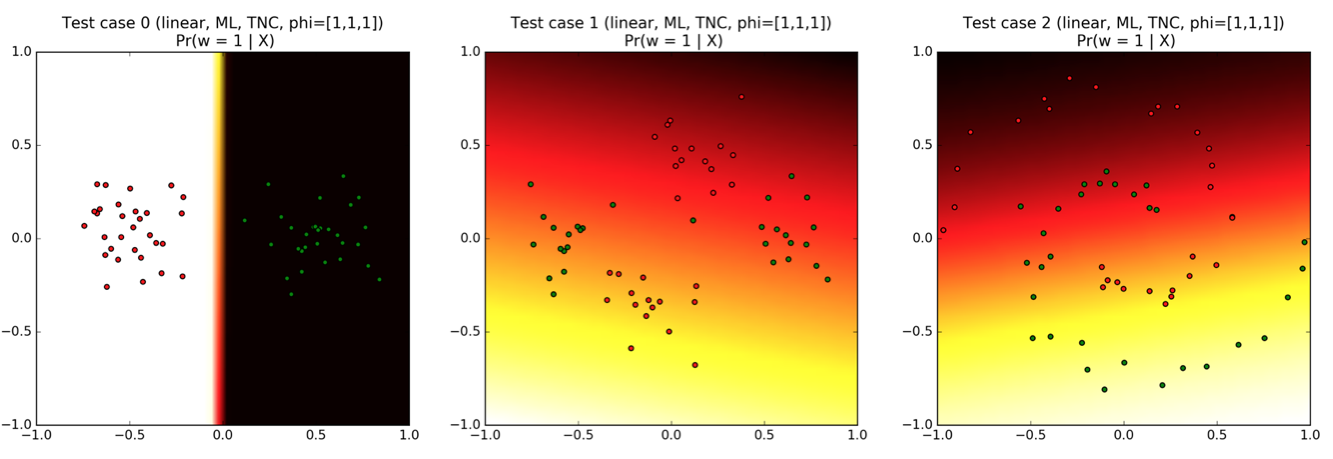
\includegraphics[width=1\textwidth]{results-lin}
    \caption{Linear logistic regression on the three datasets using ML estimates.}
  \label{fig:results-lin}
\end{figure}

We first look at some linear classifiers with the given datasets. We obtained a near perfect classifier split on \textit{test case 0}. This is an expected behaviour as there is no overlap between the two classes, so the best that we can to do is to perfectly divide the two class with a decision boundary. In \textit{test cases 1 and 2}, the data becomes intercepted and of a spiral formation. It makes it difficult to discern between the classes, where a linear model cannot deal with such cases inherently. We see in \autoref{fig:results-lin} that the trained classifier is not able to learn the seperation between classes correctly, making them poor representation of the data.

\begin{figure}[H]
  \centering
  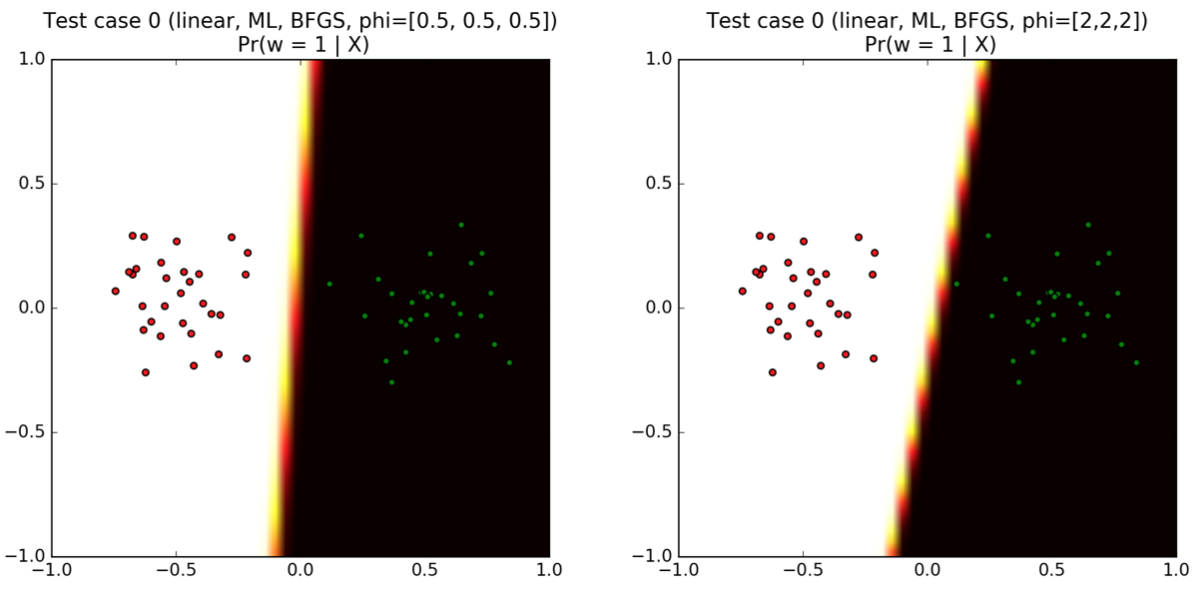
\includegraphics[width=0.9\textwidth]{tnc-comp}
    \caption{As the initial setting of $\boldsymbol\phi$ increases, the graident becomes less steep. This can be seen especially in BFGS.}
  \label{fig:tnc-comp}
\end{figure}

The initial value for $\boldsymbol\phi$ seems to be crucial as it influences the boundary in methods such as BFGS and TNC. By tweaking the initial $\boldsymbol\phi$, we observe that the estimated value changes, hence giving a different gradient to the outcome, as seen in \autoref{fig:tnc-comp}.

The advantage of MAP over ML is that MAP takes into account some prior to account for uncertainty. In \autoref{fig:ml-map-comp}, we can see that the boundary on the MAP estimated classifier is less obvious. By doing so, the model becomes less overconfident, which should provide a better result.

\begin{figure}[H]
  \centering
  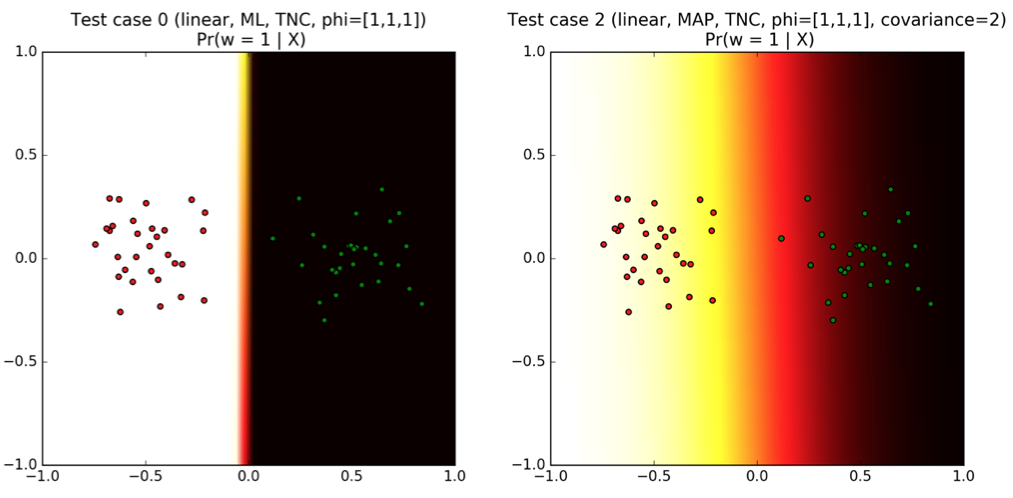
\includegraphics[width=0.9\textwidth]{ml-map-comp}
    \caption{ML estimates are used on the left and MAP estimates on used on the right. It can be observed that the right classifier has taken into account the prior, which makes the decision boundary less prominent.}
  \label{fig:ml-map-comp}
\end{figure}

\begin{figure}[H]
  \centering
  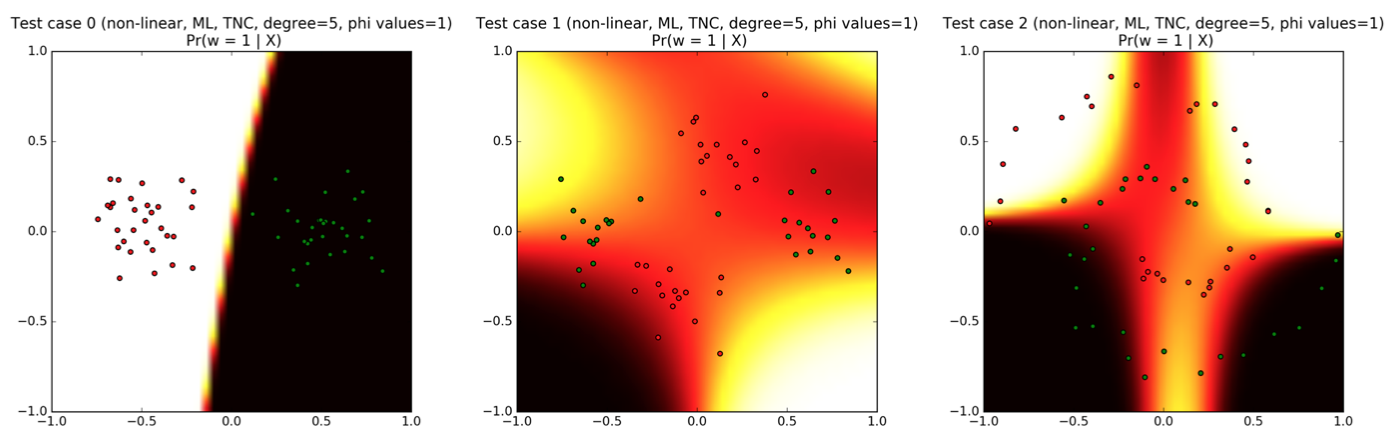
\includegraphics[width=0.9\textwidth]{results-nonlin}
    \caption{A model is trained using a degree-5 polynomial transfromation for each of the given datasets. It generated much better results on complex overlapping datasets compared to the linear ones.}
  \label{fig:results-nonlin}
\end{figure}

By transposing each 2-dimensional datapoint into 5 degrees gives models shown in \autoref{fig:results-nonlin}. We can see that the model was able to capture of of the overlapping data than the linear model. We can also see that there are overconfidence occuring because ML is used, especially in the model trained for \textit{test case 2}.

However, we can still see that simply using a non-linear method does not handle overlapping and spiral situations. Boosting can be used to help with that. With an iterative process using a Heaviside function, one can create many `weak classifiers' and combine them to form a better region that represents a class. This is useful for an overlapping situation.


% \begin{figure}[H]
  % \centering
  % 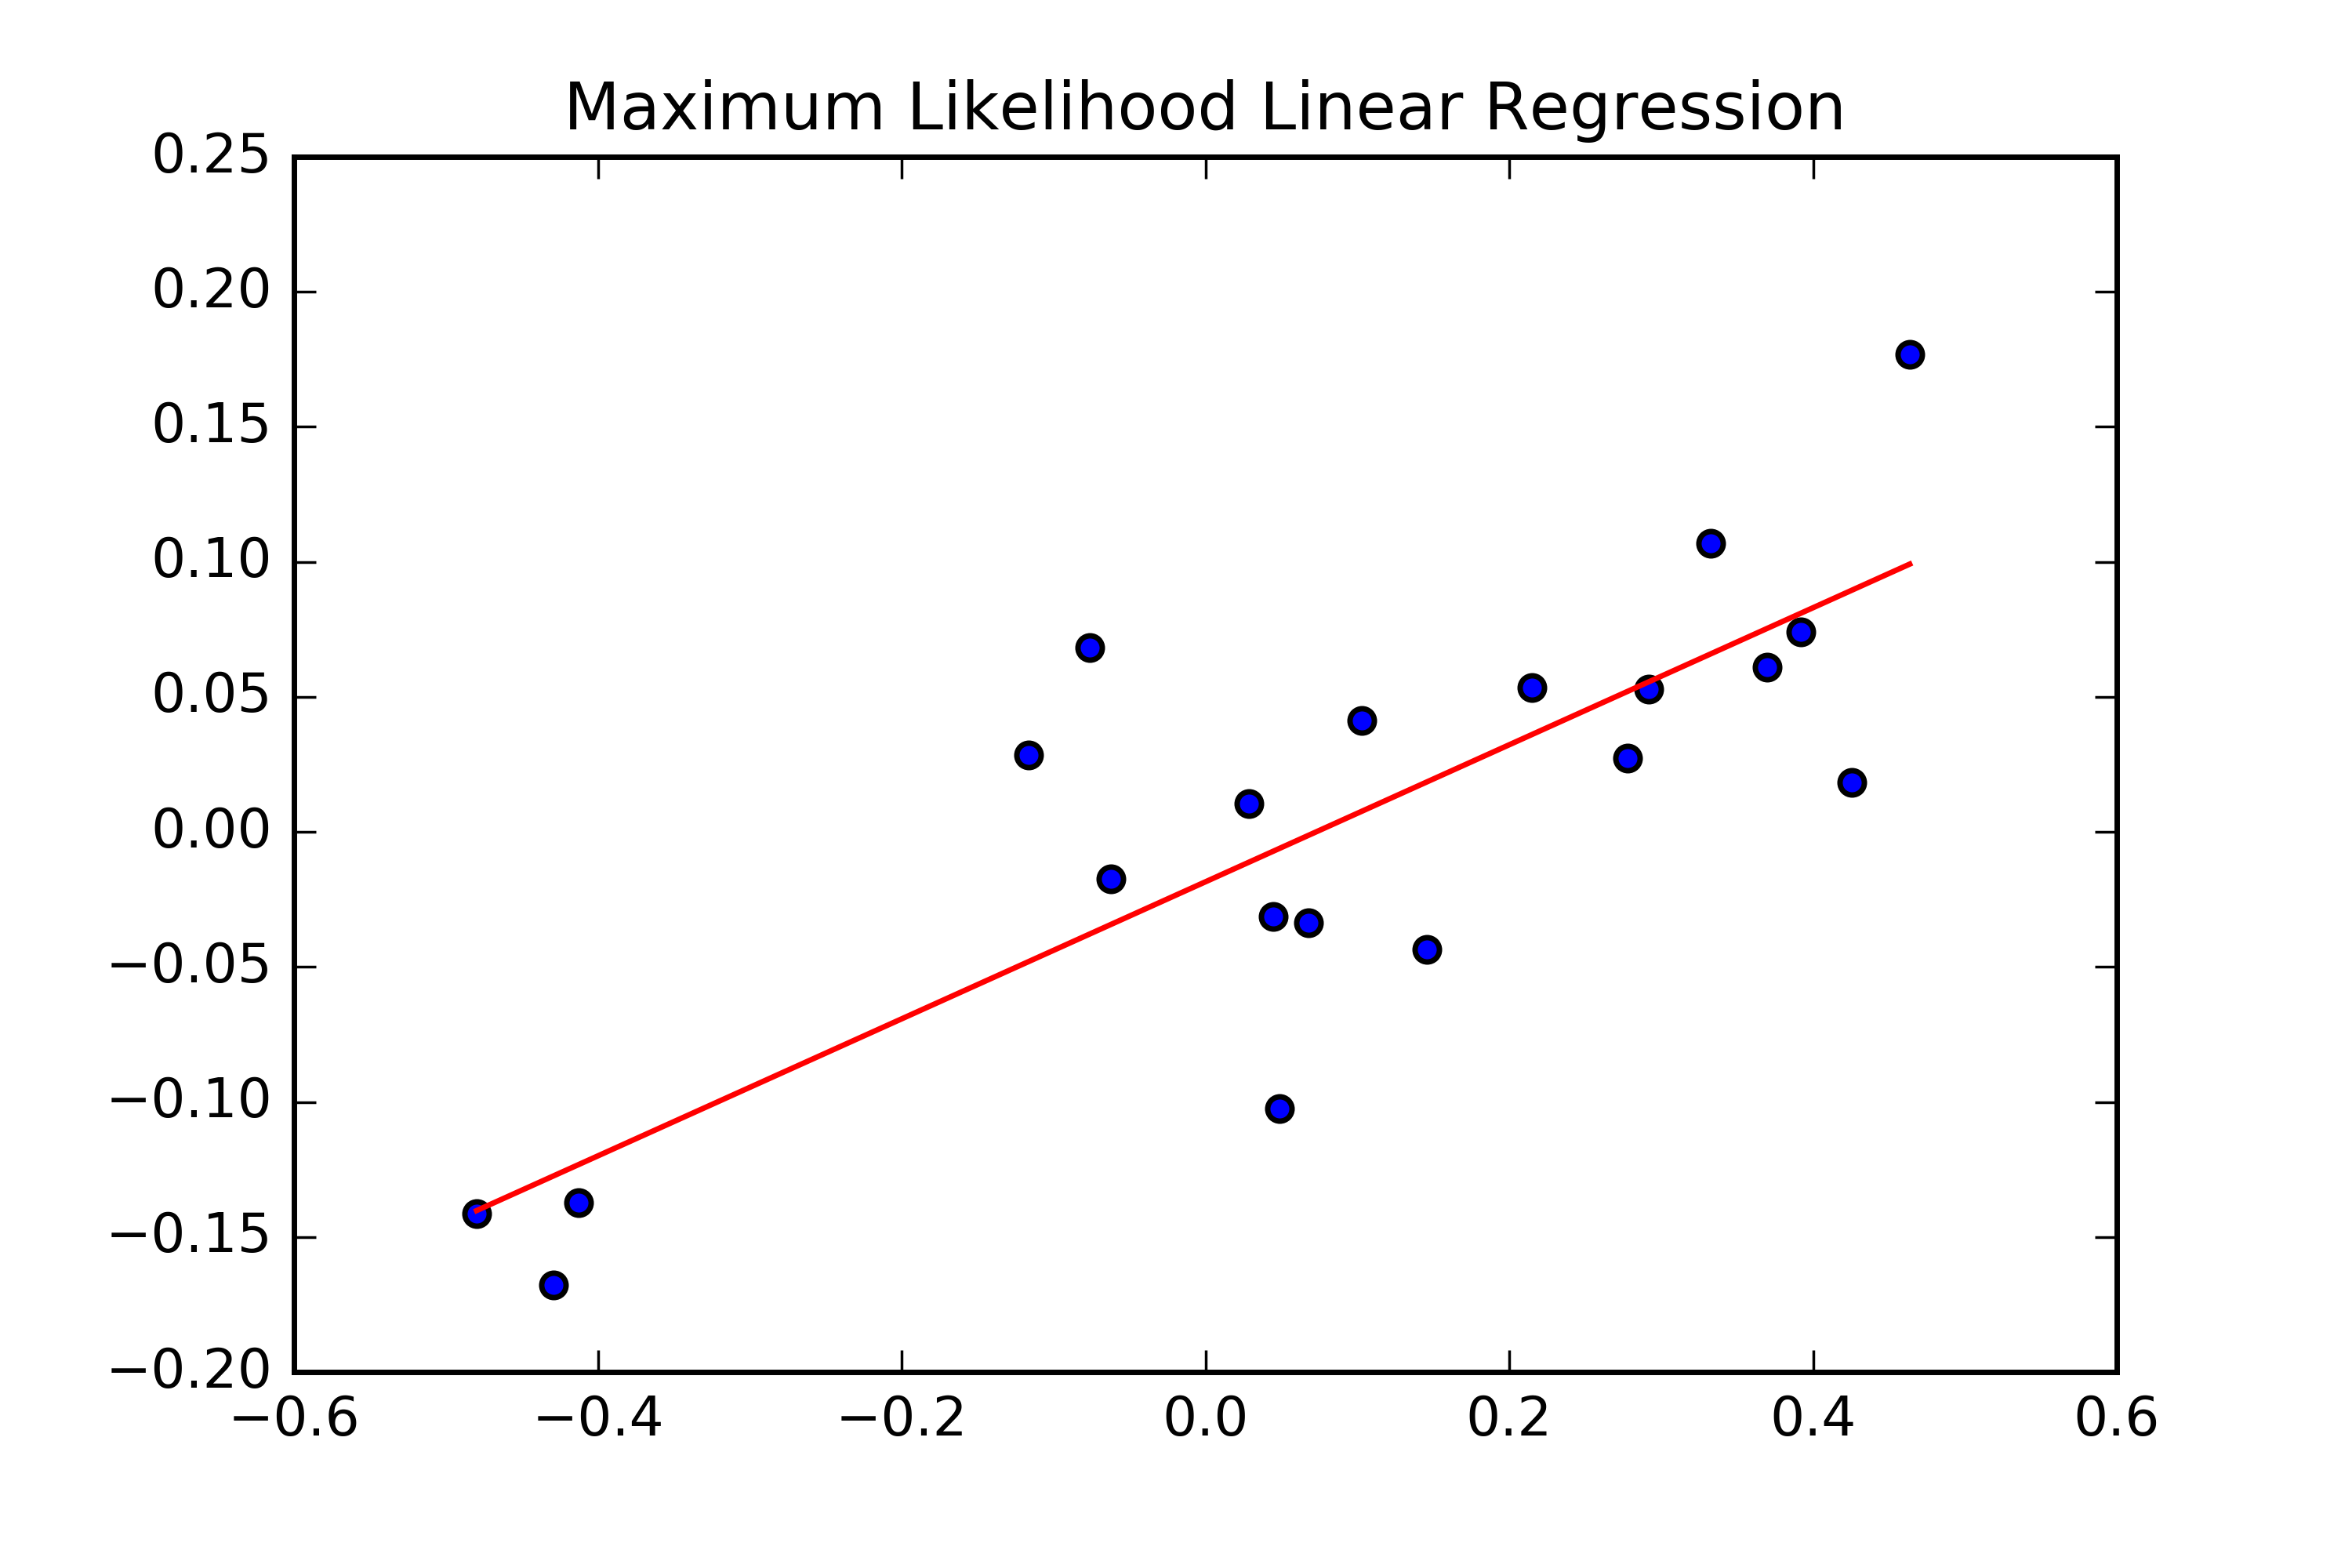
\includegraphics[width=0.7\textwidth]{lin-ml}
    % \caption{Linear regression with Maximum Likelihood parameter estimation.}
  % \label{fig:lin-ml}
% \end{figure}


% \printbibliography

\end{document}
